\documentclass{article}
\usepackage[a4paper, margin=1in]{geometry}
\usepackage{graphicx}
\usepackage{setspace}
\usepackage{booktabs}
\usepackage[utf8]{inputenc}

\begin{document}

% ================================
% COVER PAGE
% ================================
\begin{titlepage}
    \centering
    \vspace{2cm}
    
    % Title
    {\huge \textbf{Spam Detection Model}}\\[1.5cm]
    
    % Course Name
    {\large \textbf{COMP 333: Data Analytics}}\\[0.5cm]
    
    % Instructor Name
    {\large Instructor: Dr. Yaser Esmaeili Salehani}\\[1.5cm]
    
    % Submitted by
    {\large \textbf{Submitted by:}}\\[0.5cm]
    \begin{large}
        Matteo Robidoux\\
        Student ID: 40282589\\[0.5cm]
        Raagav Prasanna\\
        Student ID: 40282749\\[1.5cm]
    \end{large}
    
    % Date
    {\large \textbf{Date:}}\\[0.5cm]
    \begin{large}
        April 7th, 2025\\[1.5cm]
    \end{large}
    
    \vfill
    
    {\large Concordia University}
    
\end{titlepage}

% ================================
% ABSTRACT (start on new page)
% ================================
\newpage
\begin{abstract}
\noindent    
This study looks into the problem of finding spam in different types of input, such as SMS, email, and YouTube comments. Traditional spam detection commonly employs basic models like text vectorization. However, our study indicates that the identification of URLs embedded within messages plays a critical role in determining spam likelihood. Therefore, in addition to conventional text-based training approaches, we introduced a separate URL-based model to enhance prediction accuracy.
\newline
\newline
Furthermore, we observed key differences across input datasets. SMS messages consist solely of a body containing text, whereas emails include a subject line. Moreover, YouTube comments also often contained spam related to self-promotion, with messages similar to “Please subscribe to my channel”. Additionally, emails and comments provided unique attributes, such as email subjects and the authors of comments, which are also key pieces of data required to identify spam.
\newline
\newline
To address these variations, we developed three specialized models for SMS, email, and comment spam detection, each catering to the different datasets that we acquired. The individual model’s predictions were then combined with the output of the URL spam model whenever a URL was present. This hybrid approach significantly improved classification accuracy, achieving 99.98\% accuracy for the URL model, 96.43\% for SMS, 97.04\% for email, and 93.70\% for YouTube comments, significantly outperforming or offering similar results to traditional methods, especially when it comes to the SMS model. This study demonstrates the importance of URL detection in spam classification, and shows that a hybrid approach can effectively address the limitations of traditional spam detection methods.
\end{abstract}

% ================================
% Introduction
% ================================
% \newpage
\section{Introduction}
The rise of digital communication has led to an increase in the amount of unwanted and potentially harmful spam messages across various platforms. This includes SMS messages, emails, and content within online comment sections. Spam messages can range anywhere from harmless advertisements, to phishing attempts and even malware distribution. This emphasizes the need for effective spam detection, which is needed for ensuring the security of a user, as well as the integrity of a platform. The traditional spam detection techniques, commonly known as "ham or spam", often rely solely on text based models, using a TF\_IDF Vectorizer in conjunction with an algorithm such as SVM, Random Forest, Decision Tree, KNN, or even Naive Bayes. While these methods are effective when used to identify many different spam messages given the right input dataset, they often fail to account for additional information catering to the input, leading to both false negatives as well as false positives. In short, on many occasions, messages that are not spam are marked as spam, and messages that are, are not.
\newline
\newline
One key aspect of spam identification that is not present within traditional methods is the identification of URLs. Many spam messages contain malicious links, requiring models to take these links into account. Furthermore, a message can also contain a valid url sent from a valid user, which means that messages containing urls should not be marked as spam simply because they contain a url. Instead, the url itself should be analyzed to determine whether or not it is spam. Our study demonstrates that having a hybrid prediction approach, having one model predict the spam likelihood of a url, and having another model predict the spam likelihood of the text body, significantly improves the ability to detect spam messages when there is a url present in the body.
\newline
\newline
Moreover, spam characteristics differ across various platforms. SMS messages primarily consist of just text, whereas emails include components like subject lines. YouTube comments, on the other hand, often involve engagement-driven spam, such as self-promotion; as well as peculiar author names that could indicate spam. These differences require the need to develop specific models for each input type, as opposed to just one model.
\newline
\newline
To address these challenges, we propose a hybrid spam detection algorithm consisting of three specialized models for SMS, email, and YouTube comments. Each model is designed to identify the unique characteristics of its respective dataset, while utilizing a separate independent model for the embedded URLs in the event they exist. When a message contains a URL, the URL model’s prediction is combined with the text model’s prediction, to determine whether the message is spam. Our results demonstrate that this approach significantly enhances detection accuracy, outperforming traditional methods.
\newline
\newline
The rest of this paper is organized as follows: Section 2 reviews related work in spam detection. Section 3 describes our methodology, including dataset preprocessing, model architectures, and training procedures. Section 4 presents our experimental results and evaluation metrics. Finally, Section 5 discusses key findings, limitations, and potential future improvements.


% ================================
% Related Work
% ================================
\section{Related Work}
Spam detection has been extensively studied across various communication platforms, including SMS, emails, and online comments. Traditional spam detection approaches, as mentioned previously, use vectorization techniques such as TF-IDF, where all of the English stop words are removed from the text and only the necessary keywords remain for training; in conjunction with algorithms such as Random Forest, Naive Bayes, SVM, etc.
\newline
\newline
A notable study by Gupta et al. follows the conventional ham or spam detection algorithm using TF-IDF vectorization [1]. Their research applies machine learning models to the UCI SMS Spam Collection dataset [2], using text-based features extracted from SMS messages. Their results show strong performance in spam classification, using traditional approaches such as Naïve Bayes and SVM, emphasizing that this is an effective technique.
\newline
\newline
Another study by Gawai and Salunke [8] compared the use of various different NLP and machine learning techniques to classify SMS messages as either spam or ham, specifically for the algorithms SVM, Decision Tree, Random Forest, KNN and Naive Bayes. Their study demonstrates the effectiveness of these approaches in improving spam detection accuracy, concluding that the Naive Bayes had the most successful results, achieving an accuracy of 98\% on the UCI SMS Spam Collection dataset. They also report quite good accuracy results for the rest of the models, with 97\% for SVM, 96\% for Decision Tree, 97\% for Random Forest, and 95\% for KNN. This shows that traditional methods are still very effective when it comes to spam detection, especially when the dataset is large enough.
\newline
\newline
However, while training models on the same dataset [2], we identified a significant limitation in the way spam messages were labeled, especially when a URL was present in the message body. The dataset shows a strong bias, as many SMS messages containing URLs are labeled as spam. This introduces a risk that models trained on this data may incorrectly generalize, leading to a high false positive rate for messages containing legitimate URLs, significantly impacting simple sms messages such as a getting sent a video link from a friend. Consequently, SMS messages may be disproportionately influenced by the presence of a URL rather than the actual content of the message.
\newline
\newline
This observation highlights a critical shortcoming of traditional text-based spam detection models, being the lack of a dedicated mechanism for evaluating URLs. Our solution resolves this issue by introducing a separate URL-based classification model, which is then used in conjunction with either the SMS message model, Email model, or YouTube comments model, to predict whether they are spam. By independently determining the likelihood of a URL being spam, this hybrid approach reduces dataset bias and ensures more balanced spam classification, particularly for messages containing URLs.	

% ========== CONTINUE BELOW HERE ===============

\section{Methodology}


\subsection{Datasets and Preprocessing}

For this study, in order to ensure that each of the models have more than enough data to train and eventually perform inference on, we used a wide variety of different datasets. Specifically, we used datasets for URLs, SMS messages, Emails, and YouTube comments

\subsection*{URL Dataset}

For the URL’s we decided to have a dedicated dataset containing plenty of addresses that were classified to be either spam or non spam. This way, the model had more than enough data to decide which urls were malicious, preventing common links such as from platforms like YouTube and TikTok from being marked as spam. The kaggle dataset that we used, titled Malicious and Benign URL’s [3], contained over 450,000 url’s, that were marked as either being 0 for benign, or 1 for malicious. 


\noindent
In terms of preprocessing, we modified the names of the result and url columns to is\_spam and text respectively. Furthermore, we dropped all other columns as these were the only 2 that were needed. Additionally, we balance the dataset by dropping some urls, ensuring that there are equal number of malicious and benign urls. This is done using random samples. Finally, we normalized the text column by removing trailing whitespaces, as well as non unicode characters identified by \textquestiondown .

\begin{table}[htbp]
    \centering
    \caption{URL Dataset post Preprocessing}
    \begin{tabular}{lll}
    \toprule
     & text & is\_spam \\
    \midrule
    0 & https://www.google.com & 0 \\
    1 & https://www.youtube.com & 0 \\
    2 & https://www.facebook.com & 0 \\
    \multicolumn{3}{c}{\vdots} \\ % Represents the ellipsis
    410975 & http://mytorsmired.ru/gate.php & 1 \\
    410976 & http://narbit.com/rss/feed/stream/ & 1 \\
    410977 & http://narbit.com/rss/feed/stream & 1 \\
    \bottomrule
    \end{tabular}
    \label{tab:csv_sample}
\end{table}

\subsection*{SMS Datasets}
For SMS messages, we utilized 2 datasets being the UCI SMS Spam Collection Dataset [2], containing a total of 5575 messages, as well as another kaggle dataset named SMS SPAM DATASET [4], containing 10286 messages. Both datasets contained the headers v1 and v2, where v1 categorized the row as either ham or spam, and v2 contained the text of the SMS message.

\begin{table}[htbp]
    \centering
    \caption{UCI SMS Spam Collection Dataset}
    \begin{tabular}{lll}
    \toprule
     & v1 & v2 \\
    \midrule
    0 & ham & Go until jurong point, crazy only in ... \\
    1 & ham & Ok lar... Joking wif u oni \\
    2 & spam & Free entry in 2 a weekly comp to win FA Cup ... \\
    \multicolumn{3}{c}{\vdots} \\ % Represents the ellipsis
    5574 & spam & WINNER!! As a valued network customer you have ... \\
    5575 & spam & Had your mobile 11 months or more? Then ... \\
    \bottomrule
    \end{tabular}
    \label{tab:csv_sample}
\end{table}

\begin{table}[htbp]
    \centering
    \caption{SMS SPAM DATASET}
    \begin{tabular}{lll}
    \toprule
     & v1 & v2 \\
    \midrule
    0 & spam & Congratulations! You've been selected for a luxury vacation getaway... \\
    1 & spam & URGENT: Your account has been compromised. Click here to reset your password immediately... \\
    2 & spam & You've won a free iPhone! Claim your prize by clicking on this link now... \\
    \multicolumn{3}{c}{\vdots} \\ % Represents the ellipsis
    9526 & ham & Okie... \\
    9527 & ham & "Aight, I'm chillin in a friend's room so text me when you're on the way" \\
    \bottomrule
    \end{tabular}
    \label{tab:csv_sample}
\end{table}

When preprocessing, we merged the two datasets into a single one, and then renamed the columns to text and is\_spam. Additonally, we also decide to remove the url's that were present in the messages, as we would be using the URL dataset to classify them. This was done by using a regex pattern to identify and remove any url's that were present in the text. Finally, we also decide to balance the dataset by ensuring that there were an equal number of spam and ham messages. This was done by removing a random sample of of the messages, until there were equal amounts of spam and ham messages. This was done to ensure that the model would not be biased towards one class or the other, as well as to ensure that the model would be able to generalize well to new data.

\subsection*{Email Dataset}

When extracting the email data, we went for a total of 2 datasets. The first kaggle dataset titled Email Spam Dataset [5], contained 3 data subsets. The second dataset was titled Spam Mails Dataset [6]. In total, these 4 csv files provided us with over 23000 rows of data. 
\newline
\newline
\noindent
For preprocessing most of the methods stayed exactly the same as prior. However now we had the added challenge of needing to extract the subject from the email. This was done through simple regex matching and adding a subject column to our normalized dataset. 


\subsection*{YouTube Comments Dataset}
For comments we used a single kaggle dataset titled YouTube Comments Spam Dataset. This dataset contained the following headers: COMMENT\_ID,AUTHOR,DATE,CONTENT,VIDEO\_NAME,CLASS, and contained 1962 rows of data.
\newline
\newline
\noindent
When preprocessing, all previous methods were also applied. Furthermore, we decided to also add the author column in the normalized dataset, as we figured that it could potentially be useful in predicting spam.

\subsection{Model Features and Training}

In this section, we discuss the specific architecture and training process of each of the four models used in our spam detection system: the URL model, SMS model, Email model, and YouTube Comments model. Each model is designed to capture specific characteristics of its respective data type while integrating with the URL classifier to improve overall accuracy.

\subsubsection{URL Model}

\subsubsection*{Feature Extraction}

We extract the following features from each URL:

\begin{itemize}
    \item Structural features
        \begin{itemize}
        \item Length of the URL, number of dots, number of query parameters, etc.
        \end{itemize}
    \item Specific keywords
        \begin{itemize}
        \item Presence of words like “reward,” “win,” “gift,” “claim,”, for spam detection.
        \end{itemize}
    \item Domain and subdomain features
        \begin{itemize}
        \item Length of the domain name, presence of suspicious top-level domains (TLDs) such as .xyz or .biz
        \end{itemize}
    \item Redirect and path features
        \begin{itemize}
            \item Presence of redirects, subdomain keywords like "auth" or "login," and path length.
        \end{itemize}
\end{itemize}

\subsubsection*{Training}

\noindent
We trained an LightGBM model (lighter alternative to XGBoost, to minimize training time), with 300 boosts per round. Additionally, we also utilized Stratified K-fold, using 5 folds in total. The model was trained on 208876 rows of data. The following hyperparameters were used: 

\begin{itemize}
    \item Objective: binary
    \item Metric: Binary Logloss
    \item Boosting type: gbdt
    \item 31 leaves
    \item Learning rate of 0.1
    \item Feature fraction of 0.7
    \item Bagging fraction of 0.7
    \item Bagging frequency of 5
\end{itemize}

\noindent
The model achieved the following results after training on a Lenovo Flex 5 Laptop with a AMD Ryzen 7 4700U Processor and 16GB of DDR4 memory, taking around 187 secs:

\begin{itemize}
    \item Average Accuracy: 98.55\%
    \item Average AUC: 99.82\%
    \item Average Precision: 99.85\%
\end{itemize} 


\begin{table}[htbp]
    \centering
    \caption{URL Model Classification Report}
    \begin{tabular}{l c c c c}
    \toprule
     & Precision & Recall & F1-Score & Support \\
    \midrule
    Legitimate & 0.98 & 0.99 & 0.99 & 104438 \\
    Spam & 0.99 & 0.98 & 0.99 & 104438 \\
    \midrule
    Accuracy & & & 0.99 & 208876 \\
    Macro Avg & 0.99 & 0.99 & 0.99 & 208876 \\
    Weighted Avg & 0.99 & 0.99 & 0.99 & 208876 \\
    \bottomrule
    \end{tabular}
    \label{tab:classification_report}
\end{table}

\noindent
Additionally, the following ROC curve, Precision-Recall curve, and confusion matrix were generated to visualize the model's performance:
\begin{figure}[htbp]
    \centering
    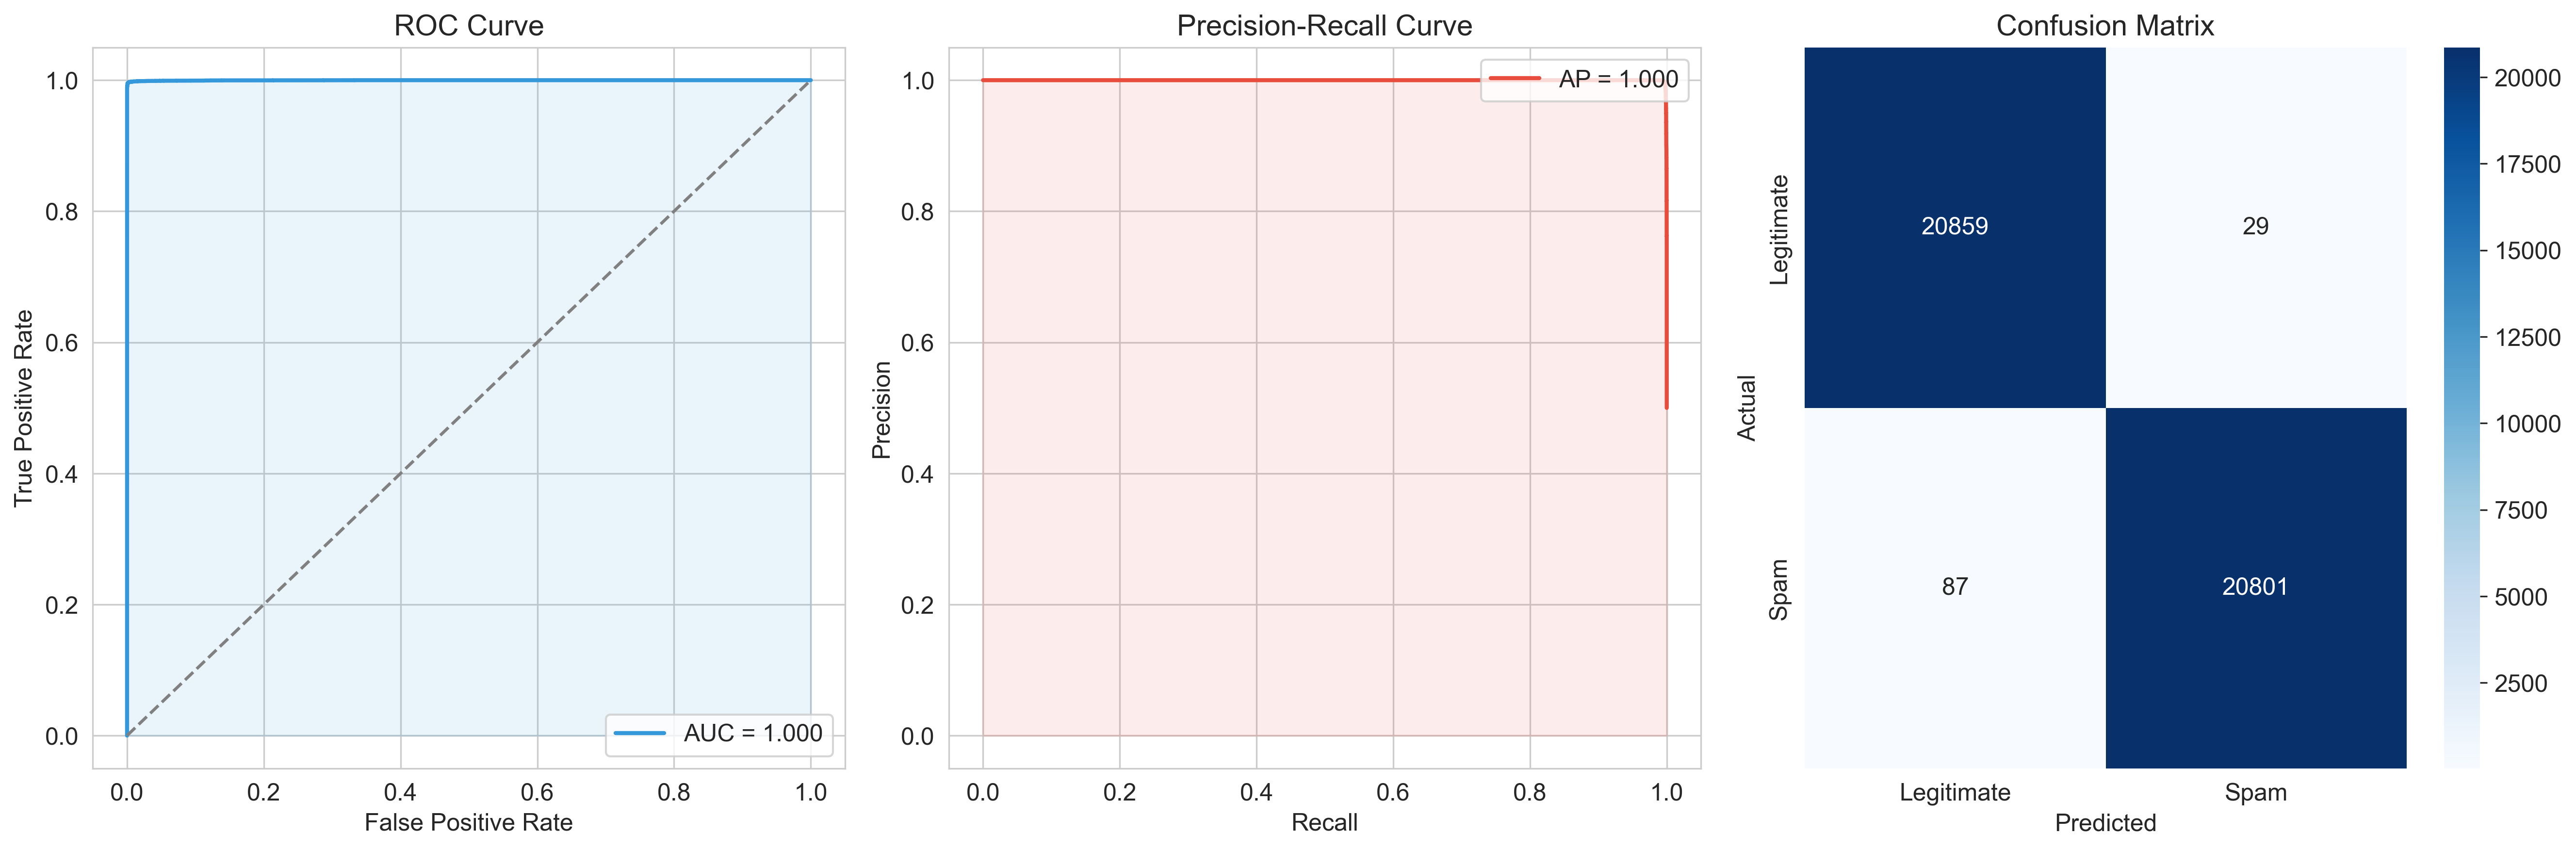
\includegraphics[width=0.8\textwidth]{../analysis/url/url_model_performance.png}
    \caption{ROC Curve, Precision-Recall Curve, and Confusion Matrix for URL Model}
    \label{fig:roc_curve}
\end{figure}

\subsubsection{SMS Model}
\subsubsection*{Feature Extraction}

We applied TF-IDF vectorization to capture word patterns and important terms while filtering out common English stopwords. The vectorization settings included:

\begin{itemize}
    \item Maximum features: 10000
    \item Minimum document frequency: 2
    \item Maximum document frequency: 0.95
\end{itemize}

\noindent
Training was done on the same laptop using Stratified K-fold with 10 folds. However this time a Random Forest Classifier was used with the following hyperparameters:

\begin{itemize}
    \item 300 estimators
    \item Max depth of 50
\end{itemize}

\noindent
The model achieved the following results after training 6306 rows, taking around 54 secs:

\begin{itemize}
    \item Accuracy: 97.02\%
    \item AUC: 99.52\%
    \item Average Precision: 99.58\%
\end{itemize}

\begin{table}[htbp]
    \centering
    \caption{SMS model Classification Report}
    \begin{tabular}{l c c c c}
    \toprule
     & Precision & Recall & F1-Score & Support \\
    \midrule
    Legitimate & 0.96 & 0.98 & 0.97 & 3153 \\
    Spam & 0.98 & 0.96 & 0.97 & 3153 \\
    \midrule
    Accuracy & & & 0.97 & 6306 \\
    Macro Avg & 0.97 & 0.97 & 0.97 & 6306 \\
    Weighted Avg & 0.97 & 0.97 & 0.97 & 6306 \\
    \bottomrule
    \end{tabular}
    \label{tab:classification_report_2}
\end{table}

\noindent
Additionally, the following ROC curve, Precision-Recall curve, and confusion matrix were generated to visualize the model's performance:
\begin{figure}[htbp]
    \centering
    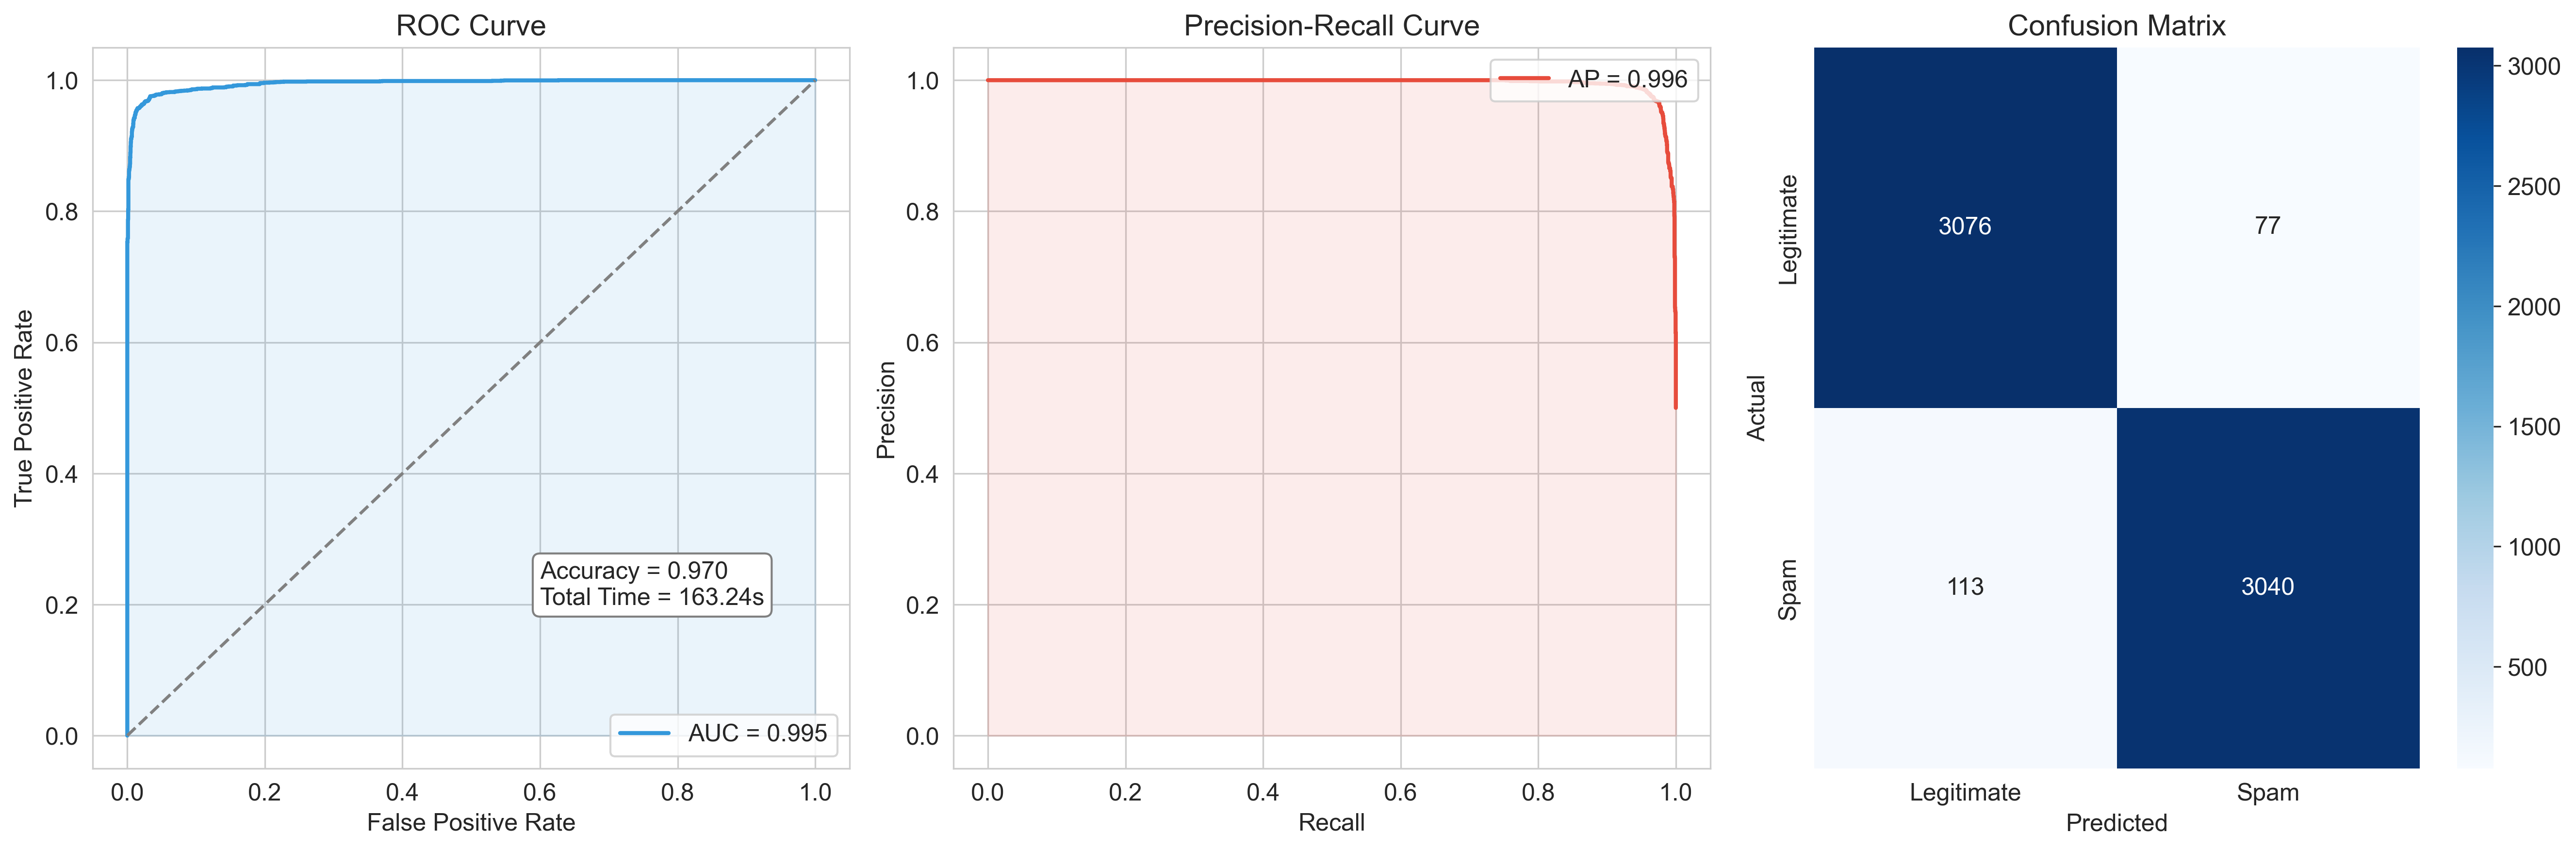
\includegraphics[width=0.8\textwidth]{../analysis/sms/sms_model_performance.png}
    \caption{ROC Curve, Precision-Recall Curve, and Confusion Matrix for SMS Model}
    \label{fig:roc_curve_2}
\end{figure}

\noindent
Furthermore, when training the model, we also decided to use another approach where we only train using the SMS UCI Spam Collection Dataset [2], using the same normalization approach (Balancing spam and non spam values, removing whitespaces, urls, etc). This was done to compare our results with the results of the study by Gawai and Salunke [8]. The model achieved the following results after training 5575 rows, taking around 17 secs: 
\begin{itemize}
    \item Accuracy: 97.12\%
    \item AUC: 99.41\%
    \item Average Precision: 99.52\%
\end{itemize}

\begin{table}[htbp]
    \centering
    \caption{SMS model Classification Report}
    \begin{tabular}{l c c c c}
    \toprule
     & Precision & Recall & F1-Score & Support \\
    \midrule
    Legitimate & 0.96 & 0.99 & 0.97 & 747 \\
    Spam & 0.99 & 0.95 & 0.97 & 747 \\
    \midrule
    Accuracy & & & 0.97 & 1494 \\
    Macro Avg & 0.97 & 0.97 & 0.97 & 1494 \\
    Weighted Avg & 0.97 & 0.97 & 0.97 & 1494 \\
    \bottomrule
    \end{tabular}
    \label{tab:classification_report_3}
\end{table}

\noindent
We also generated the following ROC curve, Precision-Recall curve, and confusion matrix to visualize the model's performance:
\begin{figure}[htbp]
    \centering
    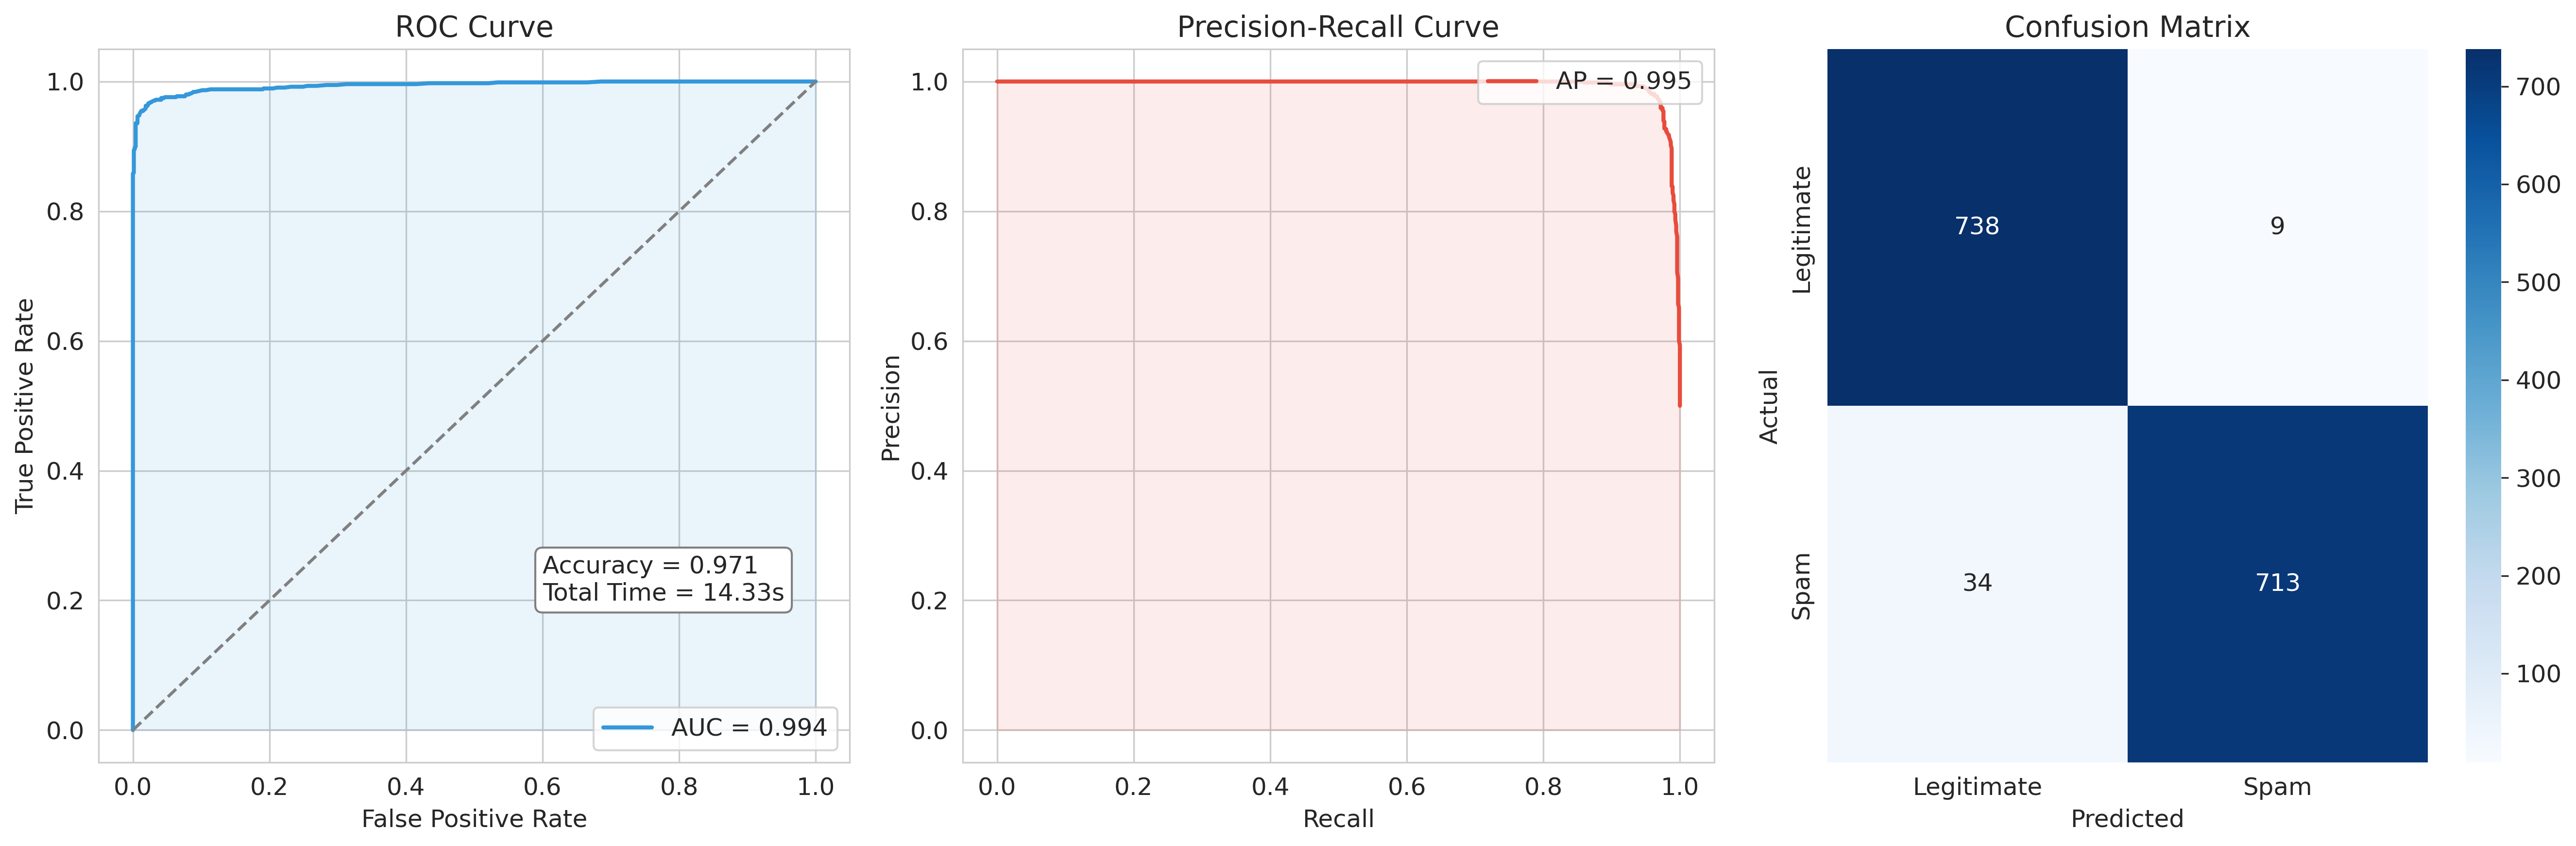
\includegraphics[width=0.8\textwidth]{../analysis/sms/sms_uci_model_performance.png}
    \caption{ROC Curve, Precision-Recall Curve, and Confusion Matrix for SMS UCI Model}
    \label{fig:roc_curve_3}
\end{figure}

\subsubsection{Email Model}
\subsubsection*{Feature Extraction}
We applied TF-IDF vectorization separately to both the email subject and body, allowing the model to leverage textual patterns in each section.

Text vectorization settings:
\begin{itemize}
    \item Minimum document frequency: 3
    \item Maximum document frequency: 0.90
    \item 5000 max features
\end{itemize}

Subject vectorization settings:
\begin{itemize}
    \item Minimum document frequency: 2
    \item Maximum document frequency: 0.95
    \item 1000 max features
\end{itemize}

\subsubsection*{Training}
We trained an XGBoost classifier (No Stratified K-fold), with the same hardware but with a 70/30 train-test split:

\begin{itemize}
    \item 500 estimators
    \item Max depth of 10
    \item Learning rate of 0.05
    \item Subsampling of 0.8
    \item Early stopping at 30 rounds if no improvement
\end{itemize}

\noindent
The model achieved the following results after training 23000 rows, taking 249 secs:

\begin{itemize}
    \item Accuracy: 96.90\%
    \item AUC: 99.59\%
    \item Average Precision: 99.55\%
\end{itemize}

\begin{table}[htbp]
    \centering
    \caption{Email Model Evaluation Report}
    \begin{tabular}{l c c c c}
    \toprule
     & Precision & Recall & F1-Score & Support \\
    \midrule
    Legitimate & 0.99 & 0.95 & 0.97 & 2649 \\
    Spam & 0.95 & 0.99 & 0.97 & 2649 \\
    \midrule
    Accuracy  & & & 0.97 & 5297 \\
    Macro Avg & 0.97 & 0.97 & 0.97 & 5297 \\
    Weighted Avg & 0.97 & 0.97 & 0.97 & 5297 \\
    \bottomrule
    \end{tabular}
    \label{tab:xgboost_evaluation}
\end{table}

\noindent
Additionally, the following ROC curve, Precision-Recall curve, and confusion matrix were generated to visualize the model's performance:
\begin{figure}[htbp]
    \centering
    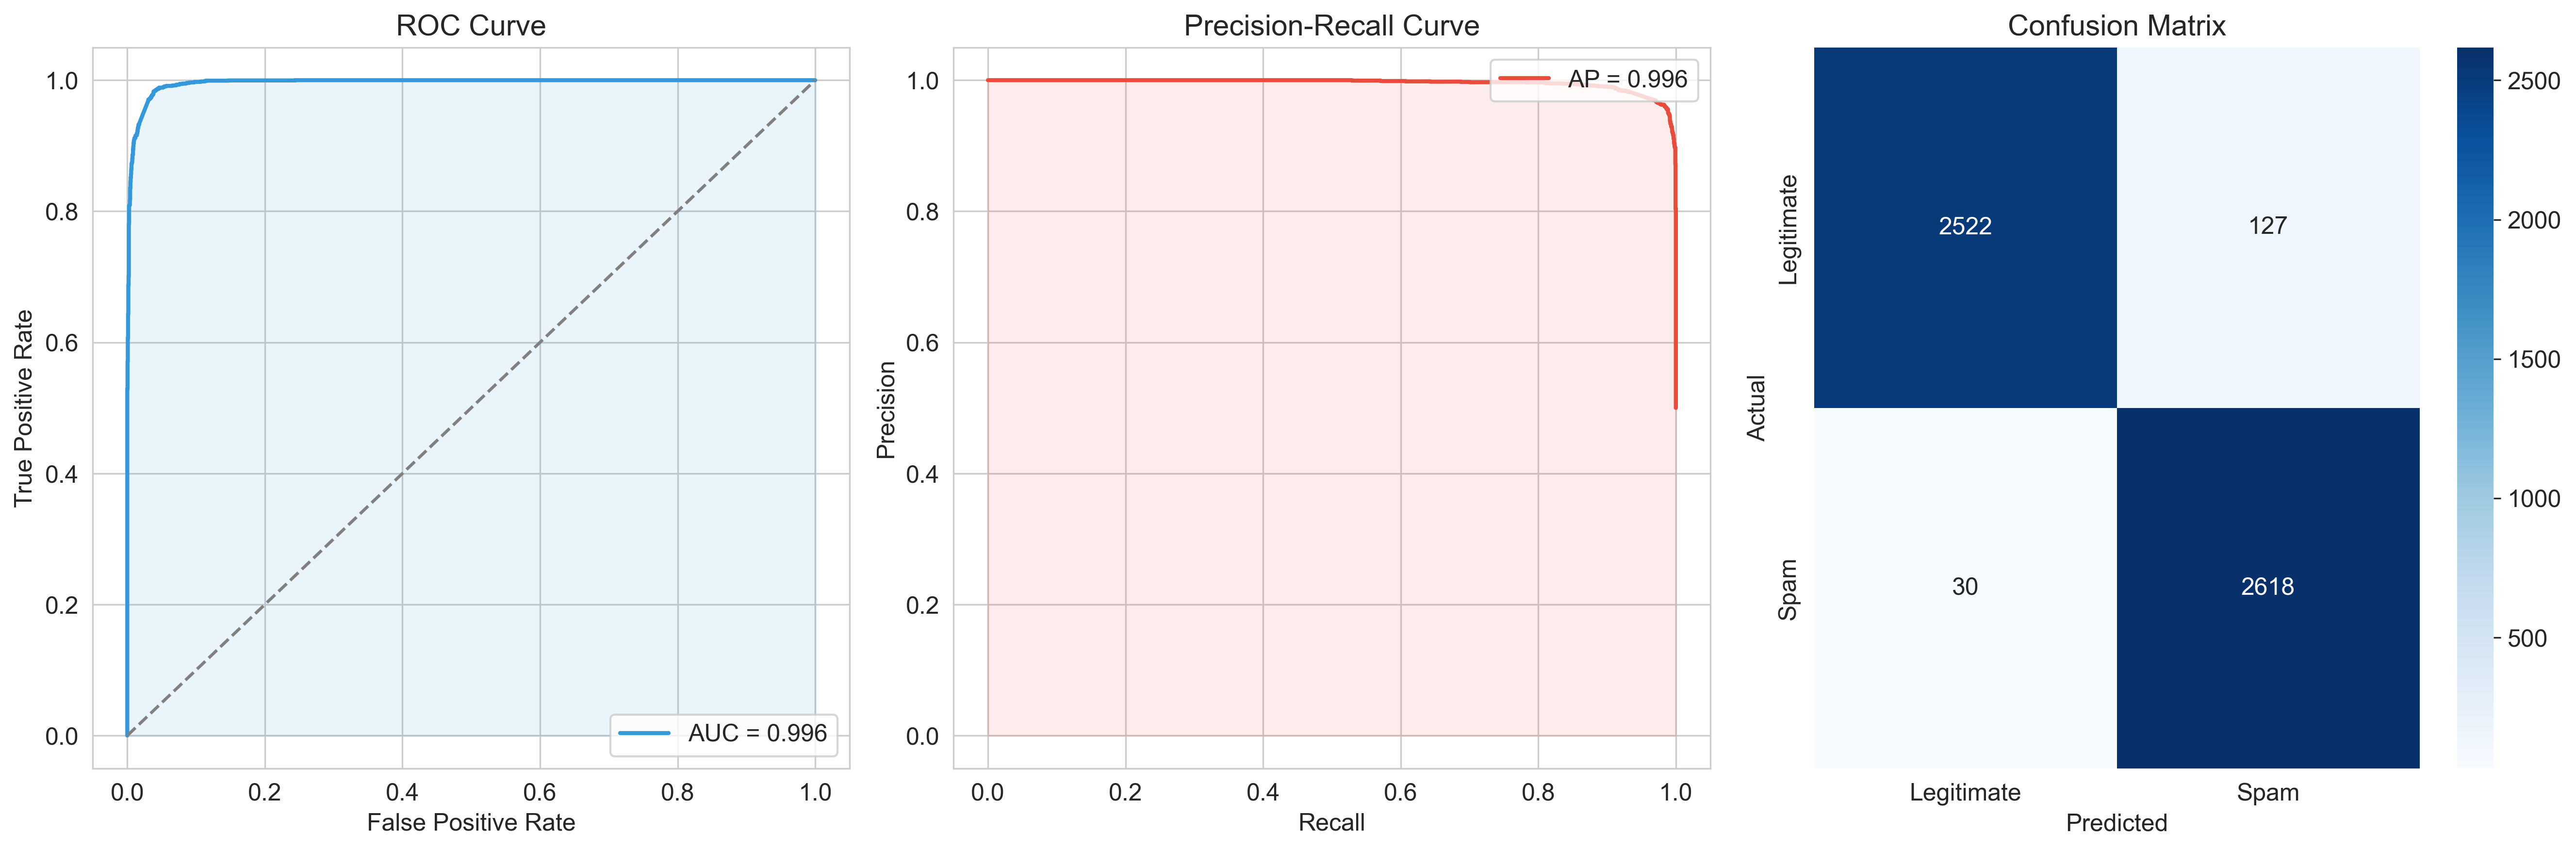
\includegraphics[width=0.8\textwidth]{../analysis/email/email_model_performance.png}
    \caption{ROC Curve, Precision-Recall Curve, and Confusion Matrix for Email Model}
    \label{fig:roc_curve_4}
\end{figure}

\subsubsection{YouTube Comments Model}
\subsubsection*{Feature Extraction}

Here we once again utilize a TF-IDF vectorizer for text, as well as one for author.

\begin{itemize}
    \item Textual Features: TF-IDF vectorization applied to comment text
    \item Author Based Features: TF-IDF vectorization applied to usernames to detect repeated spam patterns from specific users, as well as recognize patterns in usernames that look suspicious
\end{itemize}

\subsubsection*{Training}

Here we train using a Gradient Boosting Classifier mainly so we can capture hierarchical relationships within the text data, since they are comments. This is all done using the same hardware and with a 70/30 train-test split. The hyperparameters include:

\begin{itemize}
    \item 200 estimators
    \item Max depth of 5
    \item Learning rate of 0.1
    \item Subsampling of 0.8
\end{itemize}

The model achieved the following results after training 1962 rows, taking 0.75 secs:

\begin{table}[htbp]
    \centering
    \caption{Comments Gradient Boosting Model Evaluation Report}
    \begin{tabular}{l c c c c}
    \toprule
     & Precision & Recall & F1-Score & Support \\
    \midrule
    0 & 0.85 & 0.98 & 0.91 & 285 \\
    1 & 0.97 & 0.83 & 0.90 & 302 \\
    \midrule
    Accuracy & \multicolumn{4}{c}{0.90} \\
    Macro Avg & 0.91 & 0.90 & 0.90 & 587 \\
    Weighted Avg & 0.91 & 0.90 & 0.90 & 587 \\
    \bottomrule
    \end{tabular}
    \label{tab:gradient_boosting_evaluation}
\end{table}

\section{Inference}

The inference process across SMS, email, and comments, generally follows the same execution steps While the specifics vary slightly for each type of message, the overall approach remains the same.


\subsection{Preprocessing and Feature Extraction}

\begin{enumerate}
    \item URL Cleaning: Any URLs present in the text are extracted and normalized.
    \item Vectorization: The cleaned text is transformed using pre-trained vectorizers specific to each message type (SMS, email, comments). Email subjects and comment author names are also vectorized where applicable.
    \item URL Feature Extraction: If URLs are found in the text, a feature extraction function analyzes them based on characteristics such as length, presence of suspicious keywords, and domain reputation, as done within the training scripts feature extractor.
\end{enumerate}

\subsection{Probaility Estimation}

\begin{enumerate}
    \item Text Classification: The vectorized text is passed through a trained classification model that returns a spam probability score.
    \item URL Spam Detection: If URLs are present, they are sent into the URL model to predict the likelihood of them being malicious or spam-related.
    \item Weighted Combination: The probability scores from text classification and URL analysis are combined using a weighted sum approach. The weight distribution varies depending on the message type, with URL spam probability often given higher significance if URLs are detected.
\end{enumerate}

\subsection{Final Decision}

The final spam probability score is then compared against a predefined threshold (typically 0.5). If the score meets or exceeds this threshold, the message is classified as spam; otherwise, it is classified as non-spam.

\newpage

\noindent


\subsection*{References}

[1] S. D. Gupta, S. Saha, and S. K. Das, "SMS Spam Detection Using Machine Learning," *J. Phys. Conf. Ser.*, vol. 1797, no. 1, p. 012017, Feb. 2021, doi: 10.1088/1742-6596/1797/1/012017.
\newline
\newline
[2] UCI Machine Learning Repository, "SMS Spam Collection Dataset," [Online]. Available: https://www.kaggle.com/datasets/uciml/sms-spam-collection-dataset. [Accessed: 2025-03-24].
\newline
\newline
[3] S. Kumar, "Malicious and Benign URLs," [Online]. Available: https://www.kaggle.com/datasets/siddharthkumar25/malicious-and-benign-urls/data. [Accessed: Mar. 24, 2025].
\newline
\newline
[4] T. Kumar, "SMS Spam Dataset," [Online]. Available: https://www.kaggle.com/datasets/tinu10kumar/sms-spam-dataset. [Accessed: Mar. 24, 2025].
\newline
\newline
[5] N. Bharathi, "Email Spam Dataset," [Online]. Available: https://www.kaggle.com/datasets/nitishabharathi/email-spam-dataset?select=enronSpamSubset.csv. [Accessed: Mar. 24, 2025].
\newline
\newline
[6] V. Venky, "Spam Mails Dataset," [Online]. Available: https://www.kaggle.com/datasets/venky73/spam-mails-dataset. [Accessed: Mar. 24, 2025].
\newline
\newline
[7] A. Waheed, "Youtube Comments Spam Dataset," [Online]. Available: https://www.kaggle.com/datasets/ahsenwaheed/youtube-comments-spam-dataset. [Accessed: Mar. 24, 2025].
\newline
\newline
[8] S. Gawai and S. S. Salunke, "Classifying SMS as Spam or Ham Leveraging NLP and Machine Learning Techniques," in *2024 International Conference on Communication, Computing and Internet of Things (IC3IoT)*, 2024, pp. 1-6.

\newpage

\end{document}